%authentication use case

\subsubsection{Authentication}
UPRM works with sensitive and personal data therefore security plays a massive role in UPRM.
Users will be required to login with a username, password and one-time generated password. UPRM will therefore have build-in two step authentication. \\

A user will be authenticated against LDAP with their username and password. Once LDAP authentication is successful a one-time pin will be generated for the user.\\

Access rights and privileges will be set by an admin user. The admin user will have full access rights and privileges to UPRM.\\

\centerline{\fbox{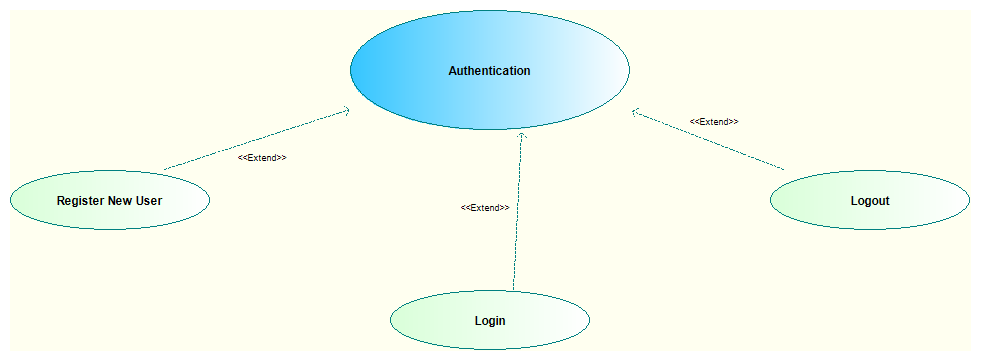
\includegraphics[width=\linewidth]{auth/OverviewAuthUseCase}}}

\subsubsubsection{Register New User\\}
Administrators and general users will already be registered on UPRM and their details will be stored on the LDAP authentication database.\\

Third party users will have to register with UPRM to gain access to the system. The details of such as user will be stored in the UPRM database.\\

\def\toclevel@paragraph{5}
\setcounter{secnumdepth}{5}
\paragraph{Use Case\\}
Register New User use case diagram.\\
\centerline{\fbox{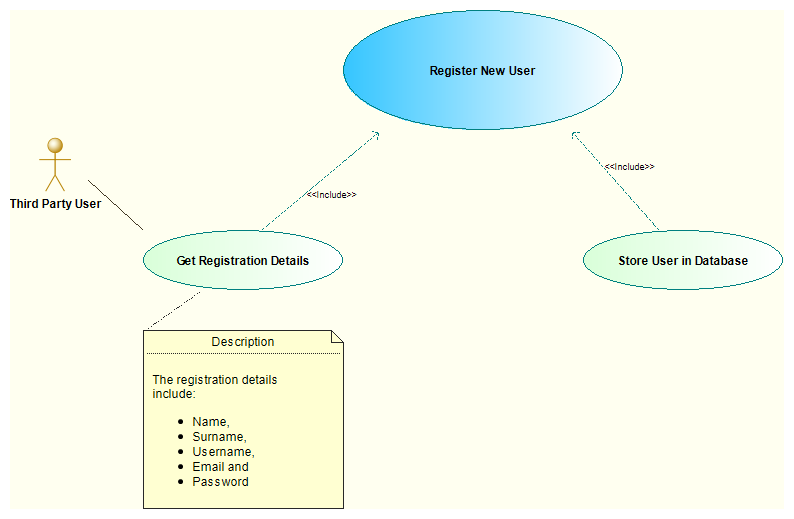
\includegraphics[width=\linewidth]{auth/RegisterNewUser}}}


\paragraph{Classes and Objects\\}



\subsubsubsection{Login\\}


\paragraph{Use Case\\}
test

\paragraph{Classes and Objects\\}


\subsubsubsection{Logout\\}

\paragraph{Classes and Objects\\}